\section{Gravitational wave detection}
\textcolor{red}{Mention initial detection summarize detections published from O1 to the end of O3.}
\\

\newpage
\subsection{The Simple Michelson interferometer}
\begin{figure}[H]
\begin{center}
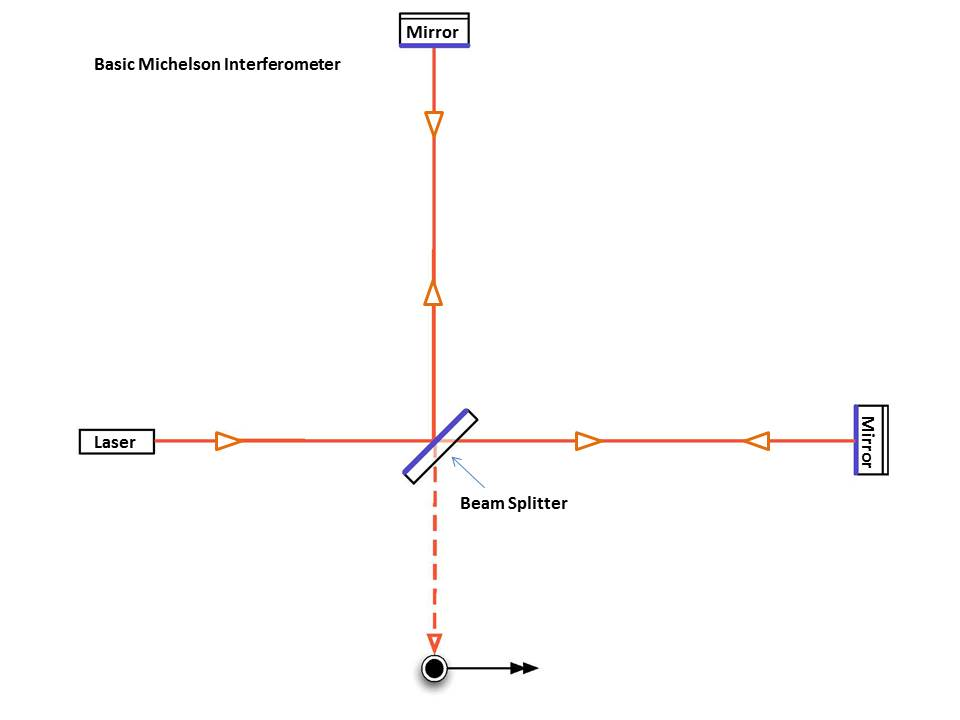
\includegraphics[width=\textwidth]{figs/INTRO/tempsub_Basic_michelson_labeled.jpg}
\end{center}
\caption{\textcolor{red}{PENDING UPDATE} The simple 4km Michelson with associated differential arm length response (left is optical schema, right is frequency response)}
\label{fig:simple_michelson}
\end{figure}

The frequency response of the Simple Michelson. Assuming a LIGO configuration (with 4km arm length), the differential arm response provides a reasonable optical gain until you reach a frequency that coorelates to a gravitational wave period $\lambda / 2$ to the interferometer arm length in such a way that the response is null.

\subsection{Fabry-Perot Michelson (FPMI)}
At the time of the proposal of LIGO, the creation of 4km long vaccum chambers was the most costly requirement for it's construction \cite{?}. When considering the possibility of constructing gravitational wave detectors, two methods for arm extension were considered: the Delay Line and the Fabry-Perot cavity. The choice ultimately became the Fabry-Perot cavity.

\subsubsection{The Fabry-Perot cavity}


\begin{figure}[H]
\begin{center}
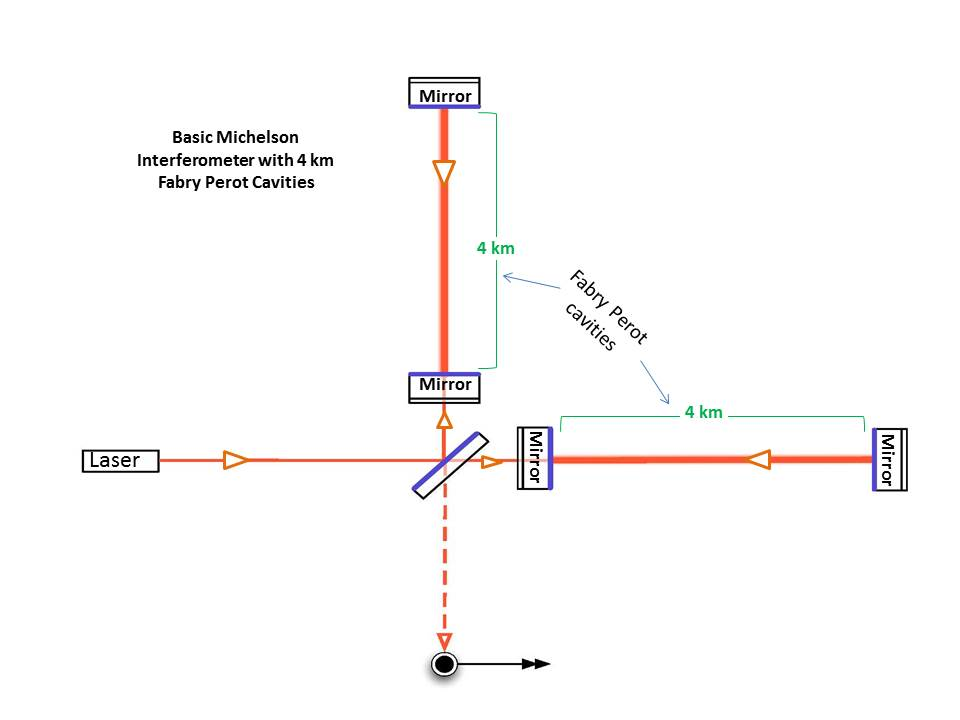
\includegraphics[width=\textwidth]{figs/INTRO/tempsub_Basic_michelson_with_FP_labeled.jpg}
\end{center}
\caption{\textcolor{red}{PENDING UPDATE} The Fabry-Perot Michelson optical schema with associated differential arm length response (left is optical schema, right is frequency response)}
\label{fig:fp_michelson}
\end{figure}

\subsection{Dual-Recycled Fabry-Perot Michelson (DRFPMI)}
Recycling mirrors are an extension of the FPMI that provide a means of enhancing the optical gain of the instrument through different means by the nature of their placement at the symmetric and anti-symmetric ports.

\begin{figure}[H]
\begin{center}
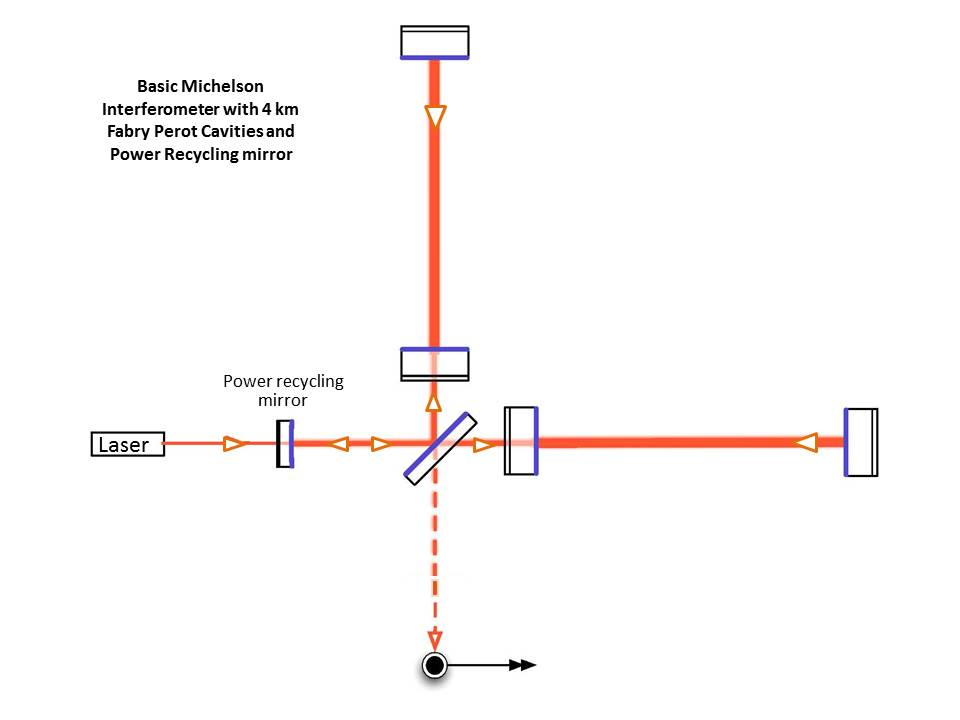
\includegraphics[width=\textwidth]{figs/INTRO/tempsub_Basic_michelson_with_FP_and_PR_labeled.jpg}
\end{center}
\caption{\textcolor{red}{PENDING UPDATE (also, borrowed figure does not have SR mirror)} The Dual-Recycled Fabry-Perot Michelson optical schema with associated differential arm length response (left is optical schema, right is frequency response)}
\label{fig:drfp_michelson}
\end{figure}


\subsubsection{Power Recycling}
When operating a FPMI, power often gets reflected back to the symmetric port leading to a significant waste of power if simply dumped. An additional partially reflective mirror is placed at said port to recirculate (or ``recycle") that power back to the arm cavities. It's positioning is kept fixed enough so that the input light adds coherently with the laser input, while the macroscopic positioning from ITMX/Y is better understood once addressing resonance and optical sidebands.

\subsubsection{Signal Recycling}
This techinique is commonly addressed to last because of it's contribution after considering the response from the PRFPMI. The principle can be understood similarly as most of the prior discussions; the use of a Fabry-Perot as an optical amplifier. By simply placing a mirror at the output port it is understood that you would take whatever light leakage coming from the PRFPMI (caused by differential arm motion) and re-introduce it to the arms. Now the question is, can that light add coherently for a signal that you are interested in detecting? As it turns out, it definitely can but careful choices must be made. Mirror location (macroscopic and microscopic tuning) as well as reflectivity have some interesting impacts to the cavity frequency response. But the general statement can be made: when introducing a mirror of relatively low reflectivity at the anti-symmetric port, you increase the detector bandwidth but at the cost of reducing the optical gain.


\section{ALIGO}
\textcolor{red}{FIGURE: Of the ALIGO config}
``Core optics" (Recycling mirrors, Beam splitter, and FP cavity mirrors) are kept suspended with quadruple pendulum suspensions so to decouple seismic activity from the mirror positions.

\subsection{Observing conditions}
The requirements for the operation of the interferometer require that the interferometer be  ``Locked"; meaning that there are some necessary configurations / criteria in order for the instrument to act as an observatory with the designed sensitivity. Cavity length and alignment stabilization as well as mode matching are some general requirements for observatory operation.

\subsubsection{Length Stabilization}
With a coupled cavity configuration, maintaining mirror positions is imperative. Techniques such as the offset lock (using a DC photodiode to measure the transmitted, reflected, or circulating power within a linear and slightly off resonance point) \cite{} and the Pound-Drever-Hall technique (reference section) are used to maintain cavity length stabilization.

\textcolor{red}{FIGURE: ALS schema?}

\subsubsection{Gaussian Beams}
So far, we've primarily discussed light and phase fronts in such a manner that hasn't addressed the important geometric constraint of using Gaussian laser light. We consider a general complex amplitude Gaussian beam propogating along the beam axis ($z$) with wavelength $\lambda$.

\begin{equation}\label{eq:gaussian_beam}
E(r) = E_o \frac{\sqrt{[\lambda z_o] / \pi}}{W(z)}e^{-r^2 / W^2(z)} e^{-ikz - ik[r^2 / (2R(z))] + i \zeta}
\end{equation}

Where $E_o$ is a complex amplitude, $r = sqrt{x^2 + y^2}$ defines the transverse beam coordinates, $k$ is the wave number, $W(z)$ is the beam width, $R(z)$ is the beam radius of curvature, and $\zeta$ is the Gouy phase.

\subsubsection{Alignment Stabilization}
\textcolor{red}{Paraxial equation}
\\
\textcolor{red}{HG modes}


\subsubsection{Mode Matching}
\textcolor{red}{LG modes}
\\
\textcolor{red}{Optical Loss}
\\
\textcolor{red}{Reduced power, Less effective squeezing}
\\
\textcolor{red}{Mention thermal compensation system (TCS) but not too much detail}

\section{Noise}

\textcolor{red}{General noise budget (LHO and LLO O3?) or just GWINC?)}

\subsection{Brownian Thermal Noise}
\textcolor{red}{Might move this section back to the $\algaas$ Electro-optic noise chapter}
\\
In 1827 the Scottish botanist Robert Brown noticed a constant motion of pollen particulates on the surface of water; witnessing randomized collisions of the water molecules holding a kinetic energy proportional to the temperature ($k_BT$) \cite{Brown:1828}. It is because of his documented observations we name the phenomena Brownian motion. And although the observations were on motion of particulates in liquids, molecules and atoms within gases and solids also exhibit Brownian motion. For high precision optical experiments operating at room temperature (and higher due to high power resonant beams), understanding how much differential phase noise is imparted on the interferometer light passing through and reflecting from core optics is crucial. This requires knowledge of the mean squared displacement from each degree of freedom of the system which can be realized through the Fluctuation Dissapation theorem. Derived by H.B. Callen and T.A. Welton, the theorem states that for a randomly fluctuating linear force \cite{Callen:1951}:

 %% Further insight into Brownian motion was explored by Einstein where he was able to relate the mean-square displacement of a particle of radius $r_\mathrm{sph}$ on a fluid with viscosity $\eta$.

 %%\begin{equation}
 %%\overline{x^2} = k_B T  \frac{1}{3 \pi \eta  r_\mathrm{sph}}
 %%\end{equation}

 %%This relation has important implications about how the random motion or fluctuations of a particulate (the pollen) is influenced (dissipated) by the viscosity of the surrounding medium (water).

\begin{equation}
F_x^2(f) = 4 k_B T\; \Re[Z]
\end{equation}

 \noindent Where $\Re[Z]$ is the real part of the impedance of the system. This impedance directly relates to equations of motion:

 \begin{equation}
 Z = \frac{F}{\dot{x}}
 \end{equation}

\noindent Another useful form is the power spectrum of the fluctuating motion:
\begin{equation}\label{fdtpsd}
x^2 (f)  = \frac{4k_B T}{(2 \pi f)^2}\; \Re[Y]
\end{equation}

Where $Y$ is the inverse of the impedance or admittance. With this power spectra, modelling and budgeting notable LIGO fundamental noise contributions attributed to the choice of the materials used for mirror substrates, and highly reflective mirror coatings becomes less daunting. Though adequate modelling of internal force couplings for the aforementioned components is required.

\subsubsection{Internal friction in Materials and Loss angle}

Zener provides a model of the internal friction of materials incorporating anelasticity into the equations of motion \cite{zener:1948}:

\begin{equation}
F = k(1+i\phi)x + m\ddot{x}
\end{equation}

Where $m$ is mass attached to a spring with a spring constant $k(1+ i\phi)$ incorporating the degree of anelasticity $\phi$. From equations 3.5 and 3.3 we perform a Laplace transform and acquire the following form of admittance:
\begin{equation}
Y(s) = \frac{\dot{x}(s)}{F(s)} = \frac{-s}{k(1+i\phi) + ms^2}
\end{equation}

\noindent Or more transparently the Fourier representation since we assume a linear time invariant system:

\begin{equation}\label{admitint}
Y(\omega) = \frac{\dot{x}(\omega)}{F(\omega)} = \frac{-i\omega}{k(1+i\phi) - m\omega^2} = \frac{k \omega \phi - i \omega (k - m \omega^2)}{(k-m\omega^2)^2 +k^2 \phi^2}
\end{equation}

\noindent Plugging equation \ref{admitint} back into \ref{fdtpsd}:

\begin{equation}
x^2 (f)  = \frac{2k_B T}{\pi}\frac{k\phi}{(k-4\pi^2 m f^2)^2 + k^2 \phi^2}
\end{equation}
Computing the admittance from a Gaussian beam impinging upon a HR mirror can require expansion of all individual mechanical degrees of freedom of the test mass system across a relevant frequency range, and with that approach convergence is not guaranteed. Saulson and Gonzalez provide an alternative method to computing the admittance coined the ``direct approach" by Levin when computing the noise from a Gaussian beam on a LIGO HR test mass. The admittance can be acquired through:

\begin{equation}\label{admitdirec}
\Re[Y] = \frac{W_\mathrm{diss}}{F_o^2}
\end{equation}

\noindent $W_\mathrm{diss}$ is the dissipated power from the system due to an oscillating force $F_o$. This form of the admittance reveals an important result of the fluctuation dissapation theorem where an undriven system with a dissapative actor, imparts motion to the degrees of freedom via a driving force by virtue of that same actor at finite temperatures. This direct approach also allows the surface pressure applied by the Gaussian beam to interrogate which mechanical modes of the test mass impose a significant energy when \ref{admitdirec} is plugged into \ref{fdtpsd}. In the case of the gaussian beam / uncoated test mass studied by Levin \cite{levin:1998}:

\begin{equation}
S_x(f) = \frac{4 k_B T}{f} \frac{1-\sigma^2}{\pi^3 E_o r_o} I\phi \bigg[1- O\bigg( \frac{r_o}{R} \bigg)\bigg]
\end{equation}

%this requires that the driving force used in a lab mimics that of a force from a centered Gaussian beam.

\textcolor{red}{Refer to Levin appendix for more on how elasticity parameters are introduced?} Where $\phi$ and $E_o$ are the Poisson ratio and Young's modulus respectively, and $O(\frac{r_o}{R})$ contains a correction term contribution as a function of the small beam radius ($r_o$) relative to the mirror radius ($R$).

\subsubsection{Coating Brownian thermal noise}
Further investigations into the beam/optic system utilizing this approach and elasticity theory led to a deeper understanding about Brownian thermal noise contributions from LIGO test masses (substrate, suspensions, HR coating). Levin mentions, with details from Harry, that the noise contributed by a lossy mirror coating is proven to be to be the most significant contributor of brownian thermal noise. Hong provides a power spectral density \cite{Hong:2013}:

\begin{equation}
S_j^X = \frac{4k_B T \lambda \phi_x^j(1- \sigma_j - 2 \sigma_j^2)}{3 \pi^2 f Y_j (1-\sigma_j)^2 \omega_o^2}
\end{equation}

Where X represents bulk and shear with j = odd (material 1) and j = even (material 2) alternating layers representing high and low index materials j = odd (material 1) j = even (material 2) for an HR coating.

\begin{figure}[H]
\begin{center}
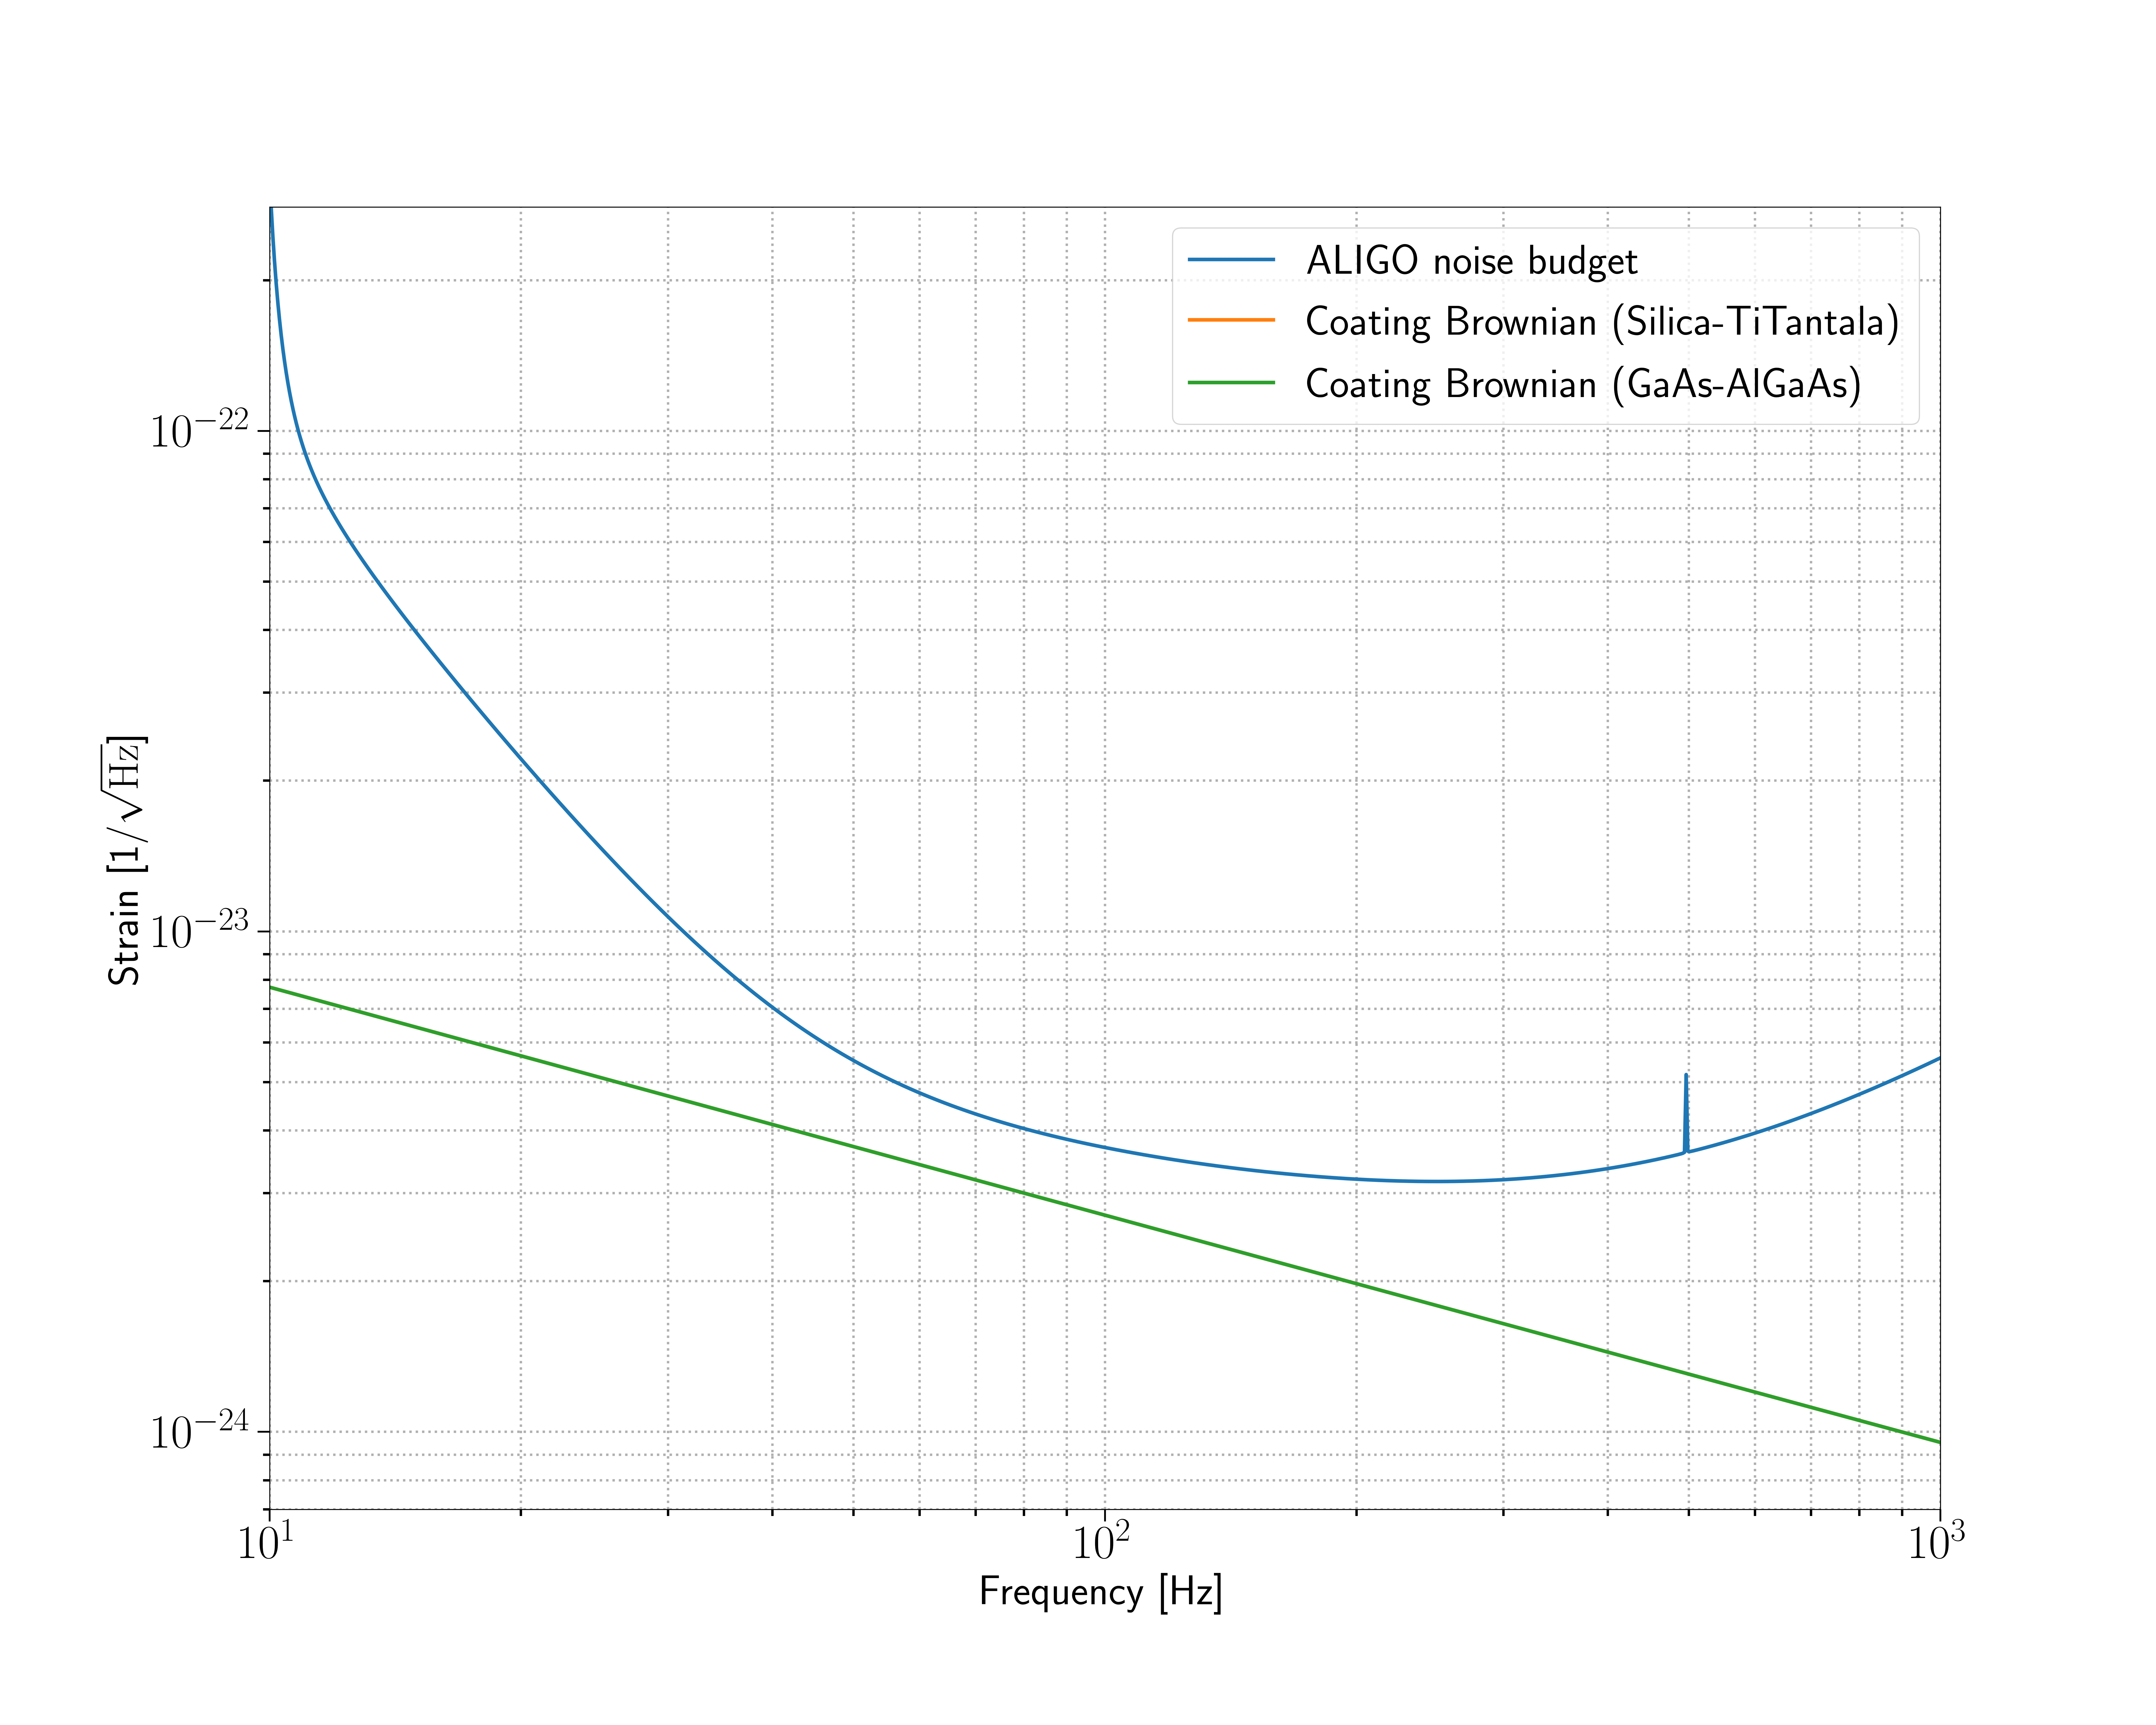
\includegraphics[width=\textwidth]{figs/ALGAAS/aligo_nb_plus_cbn.png}
\end{center}
\caption{ALIGO noise budget placeholder for silica-tantala, and gaas-algaas brownian noise comparison}
\label{fig:aligo_tn_comparison}
\end{figure}

\subsubsection{$\mathrm{SiO_2}/\mathrm{TiO_2:Ta_2O_5}$ coating parameters}
Currently the LIGO interferometers deposit $\lambda$/4 stacks of silica and titania doped tantala on fused silica test mass substrates. Effective loss angle measurements \cite{Harry:06}

\textbf{Current $\mathrm{SiO_2}/\mathrm{TiO_2:Ta_2O_5}$ elasticity params, power spectra, and strain spectral density (order of magnitude estimate)}

\subsubsection{$\gaas$/$\algaas$ coating parameters}
\textcolor{red}{Specific coating parameters for most promising $\algaas$ candidates? Chat with Steve. Or just mention parameters that are listed in Cole 2013}
\cite{Cole:2013}

\textcolor{red}{Insert computed curves of the most precise and recent (effective) loss angle measurements (Nick Demos measurements?). More instructive to plot strain spectral density or displacement power spectra}

\noindent Currently thermal noise from the $\mathrm{SiO_2}/\mathrm{TiO_2:Ta_2O_5}$ optical coatings is the largest contributor of Brownian noise in LIGO compared to estimated substrate and suspension thermal noise \cite{Harry:06}. As of the end of O3, Brownian thermal noise is estimated to be ? orders of magnitude below the current sensitivity and it will prove to be the limiting source of noise as that sensitivity is increased with various other upgrades mitigating fundamental and technical noise. (\textcolor{red}{already mentioned in intro prior to this thermal noise section. Need to re-iterate in more detail?})
